\documentclass{beamer}
\usepackage{relsize}
\usepackage{color}

\usepackage{listings}
\usetheme{CambridgeUS}
%\usepackage{beamerthemesplit} % new
\usepackage{enumitem}
\usepackage{amsmath}                    % See geometry.pdf to learn the layout options.
\usepackage{amsthm}                   % See geometry.pdf to learn the layout options. There
\usepackage{amssymb}                    % See geometry.pdf to learn the layout options.
\usepackage[utf8]{inputenc}
\usepackage{graphicx}
\usepackage[english,bulgarian]{babel}

\lstset{language=C++,
                basicstyle=\ttfamily,
                keywordstyle=\color{blue}\ttfamily,
                stringstyle=\color{red}\ttfamily,
                commentstyle=\color{green}\ttfamily,
                morecomment=[l][\color{magenta}]{\#}
}

\newtheorem{mydef}{Дефиниция}[section]
\newtheorem{lem}{Лема}[section]
\newtheorem{thm}{Твърдение}[section]

\DeclareMathOperator{\restrict}{\upharpoonright}

\setitemize{label=\usebeamerfont*{itemize item}%
  \usebeamercolor[fg]{itemize item}
  \usebeamertemplate{itemize item}}

\setbeamercovered{transparent}



\begin{document}
\title[Обектно ориентирано програмиране]{Класове, методи, this}
\author{Калин Георгиев}
\frame{\titlepage}


\begin{frame}[fragile]
\frametitle{Моделиране. Абстракция със структури от данни}


\begin{columns}[c]
  \begin{column}{0.4\textwidth}
  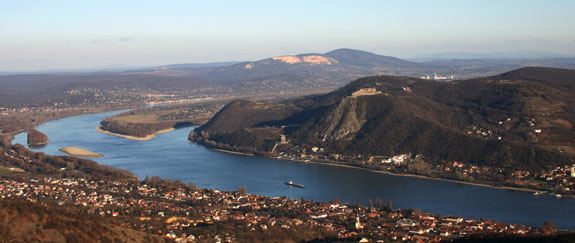
\includegraphics[width=5cm]{images/danube}
  \end{column}
  \begin{column}{0.1\textwidth}
  \relscale{4}
  $\rightarrow$
  \end{column}
  \begin{column}{0.4\textwidth}
\begin{flushleft}
\relscale{0.7}
\begin{lstlisting}
struct River
{
  char name[100];
  double waterLevels[365];
}
\end{lstlisting}
\end{flushleft}
  \end{column}
\end{columns}


\vspace{30px}

\begin{columns}[c]
  \begin{column}{0.4\textwidth}
  
\includegraphics[width=5cm]{images/people}
  \end{column}
  \begin{column}{0.1\textwidth}
  \relscale{4}
  $\rightarrow$
  \end{column}
  \begin{column}{0.4\textwidth}
\begin{flushleft}
\relscale{0.7}
\begin{lstlisting}
struct Person
{
  char name[100];
  Date birthdate;
}
\end{lstlisting}
\end{flushleft}
  \end{column}
\end{columns}


\end{frame}



\begin{frame}[fragile]
\frametitle{Логическа сигнатура}


\begin{center}
\relscale{2}
$<\mathcal{D};f_1,f_2,...,f_k;p_1,p_2,...,p_l>$
\end{center}

\begin{itemize}
  \item Носител (множество допустими стойности) -- $\mathcal{D}$
  \item Функиции (операции) -- $f:\mathcal{D}^{n}\rightarrow\mathcal{D}$
  \item Предикати -- $p:\mathcal{D}^{n}\rightarrow\{tt,ff\}$
\end{itemize}

\end{frame}


\begin{frame}[fragile]
\frametitle{Пример: Множество от букви}


\begin{center}
\relscale{2}
$<2^{\{'a'..'z'\}};\cup,\cap;empty >$
\end{center}

\begin{itemize}
  \item $A \cup B = \{x | x \in A || x \in B\}$
  \item $A \cap B = \{x | x \in A \&\& x \in B\}$
  \item $empty(A) = \left\{
  \begin{array}{ll}
    ff  & \mbox{if } \exists x \in A \\
    tt & otherwise
  \end{array}
\right.$
\end{itemize}

\end{frame}


\begin{frame}[fragile]
\frametitle{Съответна СД}


\begin{flushleft}
\relscale{0.8}
\begin{lstlisting}
struct CharSet
{
  bool contents[26];
};
\end{lstlisting}
\end{flushleft}

\begin{flushleft}
\relscale{1}
$x \in A \Leftrightarrow $
\begin{lstlisting}
A.contents[x-'a'] == true
\end{lstlisting}
\end{flushleft}

\end{frame}



\begin{frame}[fragile]
\frametitle{Съответна СД}


\begin{flushleft}
\relscale{0.8}
\begin{lstlisting}
struct CharSet
{
  bool contents[26];
};

bool empty (CharSet s)
{
  for (int i = 0; i < 26; i++)
    if (s.contents[i])
      return false;
  return true;
}
??? setUnion (????,????)
{
  ....
}
\end{lstlisting}
\end{flushleft}


\end{frame}

\begin{frame}[fragile]
\frametitle{Съответна СД}


\begin{flushleft}
\relscale{0.75}
\begin{lstlisting}
struct CharSet
{
  bool contents[26];
};
bool empty (CharSet s)
{
  for (int i = 0; i < 26; i++)
    if (s.contents[i])
      return false;
  return true;
}
CharSet setUnion (CharSet a, CharSet b)
{
  CharSet result;
  for (int i = 0; i < 26; i++)
    result.contents[i] = a.contents[i] || b.contents[i];
  return result;
}
\end{lstlisting}
\end{flushleft}


\end{frame}


\begin{frame}
\centerline{Как да обединим данните и операциите: CLASS}
\end{frame}



\begin{frame}[fragile]
\frametitle{Class}


\begin{flushleft}
\relscale{0.75}
\begin{lstlisting}
class CharSet
{
  public:
  bool contents[26];
  bool empty () //!!!
  {
    for (int i = 0; i < 26; i++)
      if (contents[i])
        return false;
    return true;
  }
  CharSet setUnion (CharSet b)
  {
    CharSet result;
    for (int i = 0; i < 26; i++)
      result.contents[i] = contents[i] || b.contents[i];
    return result;
  }
}
\end{lstlisting}
\end{flushleft}


\end{frame}


\begin{frame}[fragile]
\frametitle{class vs. struct}





\begin{columns}[t]
  \begin{column}{0.5\textwidth}
\begin{flushleft}
\relscale{0.5}
\begin{lstlisting}
class CharSet
{
  public:
  bool contents[26];
  bool empty () //!!!
  {
    for (int i = 0; i < 26; i++)
      if (contents[i])
        return false;
    return true;
  }
  CharSet setUnion (CharSet b)
  {
    CharSet result;
    for (int i = 0; i < 26; i++)
      result.contents[i] =
        contents[i] || b.contents[i];
    return result;
  }
}
\end{lstlisting}
\end{flushleft}
  \end{column}
  \begin{column}{0.5\textwidth}
\begin{flushleft}
\relscale{0.5}
\begin{lstlisting}
struct CharSet
{
  bool contents[26];
};
bool empty (CharSet s)
{
  for (int i = 0; i < 26; i++)
    if (s.contents[i])
      return false;
  return true;
}
CharSet setUnion (CharSet a, CharSet b)
{
  CharSet result;
  for (int i = 0; i < 26; i++)
    result.contents[i] =
      a.contents[i] || b.contents[i];
  return result;
}
\end{lstlisting}
\end{flushleft}

  \end{column}
\end{columns}


\end{frame}


\begin{frame}[fragile]
\frametitle{Класове / обекти}


\begin{columns}[t]
  \begin{column}{0.5\textwidth}
\begin{flushleft}
\relscale{0.75}
\begin{lstlisting}
int main ()
{
  CharSet s1,s2,s3;

  //initialization

  s3 = s1.setUnion (s2);

}
\end{lstlisting}
\end{flushleft}
  \end{column}
  \begin{column}{0.5\textwidth}
\begin{flushleft}
\relscale{0.5}
\begin{lstlisting}
class CharSet
{
  public:
  bool contents[26];
  bool empty () //!!!
  {
    for (int i = 0; i < 26; i++)
      if (contents[i])
        return false;
    return true;
  }
  CharSet setUnion (CharSet b)
  {
    CharSet result;
    for (int i = 0; i < 26; i++)
      result.contents[i] =
        contents[i] || b.contents[i];
    return result;
  }
}
\end{lstlisting}
\end{flushleft}

  \end{column}
\end{columns}


\end{frame}


\begin{frame}
\centerline{this: CharSet*}
\end{frame}




\begin{frame}[fragile]
\frametitle{this}


\begin{columns}[t]
  \begin{column}{0.5\textwidth}
\begin{flushleft}
\relscale{0.75}
\begin{lstlisting}
int main ()
{
  CharSet s1,s2,s3;

  //initialization

  s3 = s1.setUnion (s2);

}
\end{lstlisting}
\end{flushleft}
  \end{column}
  \begin{column}{0.5\textwidth}
\begin{flushleft}
\relscale{0.5}
\begin{lstlisting}
class CharSet
{
  public:
  bool contents[26];
  bool empty () //!!!
  {
    for (int i = 0; i < 26; i++)
      if (this->contents[i])
        return false;
    return true;
  }
  CharSet setUnion (CharSet b)
  {
    CharSet result;
    for (int i = 0; i < 26; i++)
      result.contents[i] =
        this->contents[i] || b.contents[i];
    return result;
  }
}
\end{lstlisting}
\end{flushleft}

  \end{column}
\end{columns}


\end{frame}


\begin{frame}
\centerline{Прости оператори}
\end{frame}

\begin{frame}[fragile]
\frametitle{Прости оператори}


\begin{center}
\relscale{1.5}
c = a.setUnion (b) $\sim$ c = setUnion (a,b)
\end{center}

\pause

\begin{center}
\relscale{1.5}
c = a + b
\end{center}

\end{frame}


\begin{frame}[fragile]
\frametitle{Прости оператори}

\begin{flushleft}
\relscale{0.8}
\begin{lstlisting}
class CharSet
{
//....
  CharSet setUnion (CharSet b){...}
};
\end{lstlisting}
\end{flushleft}

\pause

\begin{flushleft}
\relscale{0.8}
\begin{lstlisting}
class CharSet
{
//....
  CharSet operator + (CharSet b){...}
};
\end{lstlisting}
\end{flushleft}

\end{frame}



\begin{frame}
\centerline{Благодаря за вниманието!}
\end{frame}


\end{document}



\begin{columns}[t]
  \begin{column}{0.55\textwidth}

  \end{column}
  \begin{column}{0.45\textwidth}

  \end{column}
\end{columns}
